%%%%%%%%%%%%%%%%%%%%%%%%%%%%%%%%%%%%%%%%%
% Memo
% LaTeX Template
% Version 1.0 (30/12/13)
%
% This template has been downloaded from:
% http://www.LaTeXTemplates.com
%
% Original author:
% Rob Oakes (http://www.oak-tree.us) with modifications by:
% Vel (vel@latextemplates.com)
%
% License:
% CC BY-NC-SA 3.0 (http://creativecommons.org/licenses/by-nc-sa/3.0/)
%
%%%%%%%%%%%%%%%%%%%%%%%%%%%%%%%%%%%%%%%%%

\documentclass[letterpaper,11pt]{texMemo} % Set the paper size (letterpaper, a4paper, etc) and font size (10pt, 11pt or 12pt)

\usepackage{fancyhdr}
\usepackage{fancybox}
\usepackage{longtable}
\usepackage{amsmath}
%----------------------------------------------------------------------------------------
%	MEMO INFORMATION
%----------------------------------------------------------------------------------------



\memoto{Luis Andr\'es Valido Fajardo. luis.valido@umcc.cu (53694742)} % Recipient(s)

\memofrom{Josval Díaz Blanco} % Sender(s)

\memosubject{Guía de Aprendizaje para Concursantes ICPC y IOI: Búsqueda Binaria } % Memo subject

\memodate{\today} % Date, set to \today for automatically printing todays date

\logo{
\includegraphics[scale=0.5]{img/icpc}} % Institution logo at the top right of the memo, comment out this line for no logo

%----------------------------------------------------------------------------------------

%\titleguide{Detección de ciclos en un grafo}%cycle_graph
%\titleguide{Camino y ciclo de Hamilton}%hamilton_tour
%\titleguide{Encontrarse en el medio ( \emph{Meet in the Middle} )}%meet_in_middle
%\titleguide{Números Catalanes}%number_catalan
%\titleguide{Introducción al ajedrez}%introduction_chess 
%\titleguide{Permutaciones}%permutation FALTA
\titleguide{Operaciones con matrices}%matrix_operation FALTA


\begin{document}

%\AddToShipoutPicture{\BackgroundPic}
\maketitle % Print the memo header information
%\tableofcontents
\pagestyle{plain}
\pagebreak

\pagestyle{fancy}
\fancyhead[LO,CE]{ }
\fancyhead[RO,CE]{
\includegraphics[scale=0.1]{img/icpc}}
\fancyfoot[LO,CE]{\textbf{Autor:} Luis Andrés Valido Fajardo \\ \textbf{Email:} luis.valido1989@gmail.com \\ \textbf{Teléfono:} 53694742}
\fancyfoot[RO,CE]{\emph{Existen 10 tipos de personas Las que \\saben binario y LAS QUE NO}}
\fancypagestyle{plain}{\pagestyle{fancy}}



%\lhead{ }
%\rhead{  }

%\fancyfoot[L]{}
%\fancyfoot[R]{\textbf{Autor:} Luis Andrés Valido Fajardo \\ \textbf{Email:} luis.valido@umcc.cu}
%----------------------------------------------------------------------------------------
%	MEMO CONTENT
%----------------------------------------------------------------------------------------


\section{Introducción}
Una matriz es un concepto matemático que corresponde a un arreglo bidimensional en programación. Por ejemplo:

$$
  A = \begin{bmatrix}
  6	& 13 & 7 & 4 \\
  7	& 0 & 8 & 2 \\
  9	& 5 & 4 & 18
\end{bmatrix}$$

es una matriz de tamaño $3 \times 4$, es decir, tiene $3$ filas y $4$ columnas. La notación $[i, j]$ se refiere al elemento en la fila $i$ y la columna $j$ en una matriz. Por ejemplo, en la anterior matriz, $A [2, 3] = 8$ y $A [3, 1] = 9$.

Un caso especial de matriz es un vector que es una matriz unidimensional de tamaño $n \times 1$. Por ejemplo,

$$
V = \begin{bmatrix}
	4 \\
	7 \\
	5
\end{bmatrix}$$

es un vector que contiene tres elementos. De las diferentes operaciones que se pueden llevar a cabo con este concepto matemático y su implicaciones en la programación competitiva abordaremos la siguiente guía.
\section{Conocimientos previos}
\subsection{Matriz}
La matriz es un objeto o estructura matemática muy popular. Basicamente es una tabla de números con dos dimensiones. Usualmente las matrices son representadas de la siguiente manera:



$$A=\begin{bmatrix}
	a_{11} & a_{12} & \ldots & a_{1m} \\ 
	a_{21} & a_{22} & \ldots & a_{2m} \\ 
	\vdots & \vdots & \ddots & \vdots \\ 
	a_{n1} & \ldots & \ldots & a_{nm}
\end{bmatrix} $$ 

\vspace*{0.3in}

$A$ es una matriz con $n$ filas y $m$ columnas. Cada elemento en $A$ es representado como $a_{ij}$ donde $i$ es la fila enumeradas de 1 a $n$, $j$ la columna de igual forma enumeradas de 1 a $m$.

\subsection{Fórmula de Cayley}
En teoría de grafos, la fórmula de Cayley es un resultado llamado así en honor a Arthur Cayley, que establece que para cualquier entero positivo n, el número de árboles en $n$ vértices etiquetados  $n^{n-2}$. Equivalentemente, la fórmula cuenta el número de árboles de expansión de un grafo completo con vértices etiquetados. 

\subsection{Teorema de Kirchhoff}
En el campo matemático de la teoría de grafos, el teorema de Kirchhoff, nombrado por Gustav Kirchhoff es un teorema sobre el número de árboles de expansión en un grafo, mostrando que ese número puede ser computado en tiempo polinomial como el determinante de una matriz derivada del grafo. Es una generalización de la fórmula de Cayley que provee el número total de árboles de expansión en un grafo completo. 


\section{Desarrollo}
A continuación veremos algunos de los elementos y operaciones más importantes con matrices.

\subsection{Matriz cuadradra}
Una matriz es una matriz cuadrada si ella tiene el mismo número de filas y columnas. Por ejemplo, la siguiente matriz es una matriz cuadrada:

$$
S = \begin{bmatrix}
	3	& 12& 4  \\
	5	& 9 & 15 \\
	0	& 2 & 4
\end{bmatrix}$$

\subsection{Traspuesta}

La matriz traspuesta $A^T$ de la matriz $A$ se obtiene cuando las filas y columnas son intercambiadas, ejemplo $A^T[i,j] = A[j,i]$:


$$
A = \begin{bmatrix}
	6	& 13 & 7 & 4 \\
	7	& 0 & 8 & 2 \\
	9	& 5 & 4 & 18
\end{bmatrix}   
A^T = \begin{bmatrix}
6	& 7 & 9  \\
13	& 0 & 5  \\
7	& 8 & 4  \\
4	& 2 & 18
\end{bmatrix}$$

\subsection{Suma}
La suma de $A + B$ de matrices $A$ y $B$ esta definida si las matrices tienen las mismas dimensiones. El resultado es una matriz $C$ donde cada elemento $C_{i,j}$ es la suma de los correspondientes elementos en $A_{i,j}$ y $B_{i,j}$. Por ejemplo:

$$
\begin{bmatrix}
	6	& 1 & 4  \\
	3	& 9 & 2 
\end{bmatrix} +  \begin{bmatrix}
4	& 9 & 3  \\
8	& 1 & 3
\end{bmatrix} = \begin{bmatrix}
6+4 & 1+9 & 4+3  \\
3+8	& 9+1 & 2+3 
\end{bmatrix} = \begin{bmatrix}
10	& 10 & 7  \\
11	& 10 & 5 
\end{bmatrix} $$

\subsection{Multiplicación}
\subsubsection{Por un valor}

Multiplicar una matriz $A$ por un valor $x$ significa que cada elemento de $A$ es multplicado por $x$. Por ejemplo:

$$
2 \cdot \begin{bmatrix}
	6	& 1 & 4 \\
	3 & 9 & 2
\end{bmatrix}   
 = \begin{bmatrix}
 	2 \cdot 6 & 2 \cdot 1 & 2 \cdot 4 \\
 	2 \cdot 3 & 2 \cdot 9 & 2 \cdot 2
 \end{bmatrix} =
\begin{bmatrix}
	6 & 1 & 4 \\
	3 & 9 & 2
\end{bmatrix}$$

\subsubsection{Por otra matriz}

El producto $AB$ de las matrices $A$ y $B$ esta definido si $A$ tiene las dimensiones $a\times n$ y las dimensiones de $B$ es $n \times b$, es decir la cantidad de columnas de $A$ debe ser igual a la cantidad de filas de $B$ para poder efectuar la operación. La operación da como resultado una matriz $C$ de dimensiones $a \times b$ donde cada elemento es calculado usando la siguiente fórmula:

$$ AB[i,j] = \sum_{k=1}^{n}A[i,k]\cdot B[k,j] $$




La idea es que cada elemento de AB es la suma de productos de los elementos de A y B acorde a la siguiente figura:

% TODO: \usepackage{graphicx} required
\begin{figure}[h!]
	\centering
	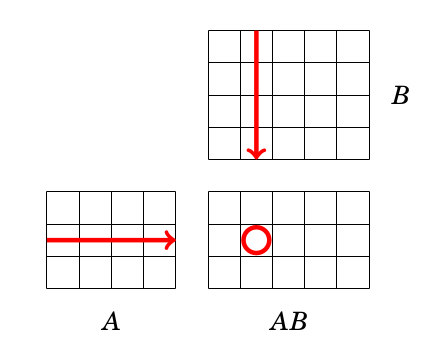
\includegraphics[width=0.5\linewidth]{img/mulmatriz}
	\label{fig:mulmatriz}
\end{figure}

Por ejemplo:
$$
\begin{bmatrix}
   1 & 4 \\
   3 & 9 \\
   8 & 6 
\end{bmatrix}
\cdot
\begin{bmatrix}
	1 & 6 \\
	2 & 9
\end{bmatrix}   
= \begin{bmatrix}
	1 \cdot 1 + 4 \cdot 2  & 1 \cdot 6 + 4 \cdot 9  \\
	3 \cdot 1 + 9 \cdot 2 &  3 \cdot 6 + 9 \cdot 9 \\
	8 \cdot 1 + 6 \cdot 2 &  8 \cdot 6 + 6 \cdot 9 
\end{bmatrix} =
\begin{bmatrix}
	9 & 42 \\
	21 & 99 \\
	20 & 102 
\end{bmatrix}$$

La multplicacion de matrices es asociativa, entonces $A(BC) = (AB)C$ es lo mismo, pero no es conmutativa es decir $AB = BA$ usualmente no es lo mismo. 


\subsection{Matriz identidad}

Una matriz identidad es una matriz cuadrada donde cada elemento de la diagonal es $1$ y todos los otros elementos son $0$. Por ejemplo, la siguiente matriz es una matriz identidad de $3\times 3$

$$
I = \begin{bmatrix}
	 1 & 0 & 0 \\
	 0 & 1 & 0 \\
	 0 & 0 & 1
\end{bmatrix}$$

Multiplicar una matriz por una matriz identidad no cambia en nada la matriz. Por ejemplo:

$$
 \begin{bmatrix}
	1 & 0 & 0 \\
	0 & 1 & 0 \\
	0 & 0 & 1
\end{bmatrix}  \cdot
\begin{bmatrix}
 1 & 4 \\
 3 & 9 \\
 8 & 6
\end{bmatrix} =
\begin{bmatrix}
	1 & 4 \\
	3 & 9 \\
	8 & 6
\end{bmatrix} \text{y} 
\begin{bmatrix}
	1 & 4 \\
	3 & 9 \\
	8 & 6
\end{bmatrix}
  \cdot
  \begin{bmatrix}
 	1 & 0 \\
 	0 & 1 
 \end{bmatrix}
 =
\begin{bmatrix}
	1 & 4 \\
	3 & 9 \\
	8 & 6
\end{bmatrix}$$ 

\subsection{Potencia}
La potencia de $A^k$ de una matrix $A$ es definida si $A$ es una matriz cuadrada. La definición esta basada en la multiplicación de matrices:

$$
A^k = \underset{\text{k veces}}{\underbrace{A \cdot A \cdot A \dots A}}
$$

Por ejemplo:

$$
\begin{bmatrix}
	2 & 5  \\
	1 & 4 
\end{bmatrix}^3  =
\begin{bmatrix}
	2 & 5  \\
	1 & 4 
\end{bmatrix} \cdot
\begin{bmatrix}
	2 & 5  \\
	1 & 4 
\end{bmatrix} \cdot
\begin{bmatrix}
	2 & 5  \\
	1 & 4 
\end{bmatrix}
=
\begin{bmatrix}
	48 & 165  \\
	33 & 114
\end{bmatrix}$$ 

En correspondencia $A^0$ es una matriz identidad. Por ejemplo:

$$\begin{bmatrix}
	2 & 5  \\
	1 & 4 
\end{bmatrix}^0  =
\begin{bmatrix}
	1 & 0  \\
	0 & 1 
\end{bmatrix}$$



La matrix $A^k$ puede ser eficientemente calculada en O($n^3\log k$) usando el algoritmo de exponenciación binaria. Por Ejemplo

$$\begin{bmatrix}
	2 & 5  \\
	1 & 4 
\end{bmatrix}^8  =
\begin{bmatrix}
	2 & 5  \\
	1 & 4
\end{bmatrix}^4 \cdot
\begin{bmatrix}
	2 & 5  \\
	1 & 4
\end{bmatrix}^4$$



\subsection{Determinante}

El determinante $det(A)$ de una matriz $A$ es definido si la matriz $A$ es cuadradada. Si las dimensiones de $A$ es $1 \times 1$, entonces $det(A) = A[1,1]$. El determinante de matrices de mayores dimensiones se calcula recursivamente usando la fórmula:

$$ det(A)=\sum_{j=1}^{n}A[1,j]C[1,j]$$

donde $C[i,j]$ es el cofactor de $A$ en $[i,j]$. El cofactor es calculado usando la fórmula:

$$C[i,j] = (-1)^{i+j}det(M[i,j])$$



donde $M[i,j]$ se obtiene por remover la fila $i$ y columna $j$ de $A$.  Debido al coeficiente $( -1)^{i+j}$ en el cofactor, todos los demás determinantes son positivos y negativos. Por ejemplo,

$$ det(\begin{bmatrix}
	1 & 4 \\
	3 & 9 
\end{bmatrix})=3 \cdot 6 - 4 \cdot 1 =14$$

y

$$ det(\begin{bmatrix}
	2 & 4 &3 \\
	5 & 1 & 6\\
	7 & 2 & 4
\end{bmatrix})=2 \cdot det(\begin{bmatrix}
1 & 6  \\
2 & 4 \end{bmatrix}) - 4 \cdot det(\begin{bmatrix}
5 & 6  \\
7 & 4 \end{bmatrix}) + 3 \cdot det(\begin{bmatrix}
5 & 1  \\
7 & 2 \end{bmatrix})  =81$$

El determinante de $A$ nos dice si existe una matriz inversa $A^{-1}$ tal que $A \cdot A^{-1} = I$ , donde $I$ es una matriz identidad. Resulta que $A^{-1}$ existe exactamente
cuando $det(A) \neq  0$, y se puede calcular usando la fórmula:

$$ A^{-1}[i,j] = \frac{C[i,j]}{det(A)}  $$

Por ejemplo:

$$ \underset{A}{\underbrace{\begin{bmatrix} 2 & 4 &3 \\ 5 & 1 & 6\\ 7 & 2 & 4 \end{bmatrix}}}
\cdot \underset{A^{-1}}{\underbrace{\frac{1}{81}\begin{bmatrix} -8 & -10 &21 \\ 22 & -13 & 3\\ 3 & 24 & -18 \end{bmatrix}}} = \underset{I}{\underbrace{\begin{bmatrix} 1 & 0 &0 \\ 0 & 1 & 0\\ 0 & 0 & 1 \end{bmatrix}}}$$


\subsection{Rango}
El rango de una matriz es el mayor número de filas/columnas linealmente independientes de la matriz. El rango no solo se define para matrices cuadradas. El rango de una matriz también se puede definir como el orden más grande de cualquier menor distinto de cero en la matriz.

Deje que la matriz sea rectangular y tenga tamaño $ N \times M $. Tenga en cuenta que si la matriz es cuadrada y su determinante no es cero, entonces el rango es $ n $ ($ = m $); De lo contrario, será menos. En general, el rango de una matriz no excede $ \min (n, m) $.

La mejor manera de entender este concepto es con un ejemplo, vamos a determinar cuántas filas o columnas son linealmente independientes en las siguientes matrices:

$$ A = \begin{bmatrix}
	1	& 2  \\
	2	& 4 
\end{bmatrix}  
B = \begin{bmatrix}
	2	& 1 & -1 \\
	0	& -1 & 2  \\
	2	& 0 & 1 
\end{bmatrix}
C = \begin{bmatrix}
	2	& 1 & 1 \\
	0	& 2 & 1 \\
	0	& 0 & -1
\end{bmatrix}    
$$

Como puedes observar en la matriz $A$, la segunda fila corresponde a la primera fila multiplicada por 2. Entonces, una fila es la combinación lineal de la otra y, por lo tanto, solo una de ellas es linealmente independiente $R_g(A) =1$. Para la matriz $B$, podemos observar que la tercera fila es la suma de la primera y la segunda fila. Las dos primeras son linealmente independientes entre sí, por lo que $R_g(B) =2$. En la matriz $C$ no hay ninguna operación entre las filas o columnas que las relacione. Por tanto, $R_g(C) =3$. 

Puede buscar el rango usando la eliminación gaussiana. Realizaremos las mismas operaciones que cuando resuelvan el sistema o encuentren su determinante. Pero si en algún paso en la columna $ i $ -th no hay filas con una entrada no vacía entre las que ya no seleccionamos, entonces saltamos este paso. De lo contrario, si hemos encontrado una fila con un elemento distinto de cero en la columna $ i $ -th durante el paso $ i $ -th, entonces marcamos esta fila como uno seleccionado, aumentamos el rango por uno (inicialmente el rango se establece igual a $ 0 $) y realiza las operaciones habituales de quitar esta fila del resto.

%Cubico

\section{Implementación}
\subsection{C++}
\begin{lstlisting}[language=C++]
#define EPS 1e-9
typedef double number;
typedef vector <number> Array;
typedef vector <Array > Matrix;

Matrix identity (int n) {
   Matrix A (n, Array (n,0));
   for (int i=0; i<n; ++i) A[i][i]=1;
   return A;
}

Matrix sum( Matrix & A,  Matrix & B){
   Matrix C (A.size(),Array(A[0].size()));
   for (int i = 0; i<C.size(); ++i)
      for (int j=0; j<C[i].size (); ++j) C[i][j] = A[i][j] + B[i][j];
   return C;
}

Matrix mul ( Matrix & A,  Matrix & B) {
   Matrix C (A.size (), Array (B [0]. size ()));
   for (int i = 0; i<C.size(); ++i)
      for (int j=0; j<C[i].size (); ++j)
         for (int k=0; k<A[i].size(); ++k) C[i][j]+= A[i][k] * B[k][j];
   return C;
}

Matrix pow (Matrix & A, int e){
   Matrix ret = identity(A.size());
   while(e){
      if(e&1) ret=mul(ret,A);
      e>>=1;
      A=mul(A,A);
   }
   return ret;
}

number det(Matrix A) {
   const int n = A.size();
   number D = 1;
   for (int i = 0; i < n; ++i) {
      int pivot = i;
      for (int j = i+1; j < n; ++j)
         if (abs(A[j][i]) > abs(A[pivot][i])) pivot = j;
      swap(A[pivot], A[i]);
      D *= A[i][i] * (i != pivot ? -1 : 1);
      if (abs(A[i][i]) < EPS) break;
      for(int j = i+1; j < n; ++j)
         for(int k = n-1; k >= i; --k) A[j][k] -= A[i][k] * A[j][i] / A[i][i];
   }
   return D;
}

int rankMatrix(Matrix A) {
   int n = A.size(); int m = A[0].size();
   int rankM = 0;
   vector<bool> row_selected(n, false);
   for (int i = 0; i < m; ++i) {
      int j;
      for (j = 0; j < n; ++j) 
         if (!row_selected[j] && abs(A[j][i]) > EPS) break;
	  if (j != n) {
         ++rankM;
         row_selected[j] = true;
         for (int p = i + 1; p < m; ++p) A[j][p] /= A[j][i];
         for (int k = 0; k < n; ++k) {
            if (k != j && abs(A[k][i]) > EPS) {
               for (int p = i + 1; p < m; ++p) A[k][p] -= A[j][p] * A[k][i];
            }
         }
      }
   }
   return rankM;
}

\end{lstlisting}

\subsection{Java}

\begin{lstlisting}[language=Java]
public class Main {
   private double EPS = 1e-9;
	
   public double[][] identity(int n) {
      double[][] A = new double[n][n];
      for (int i = 0; i < n; ++i) { Arrays.fill(A[i], 0); A[i][i] = 1;}
      return A;
   }
	
   public double[][] sum(double[][] A, double[][] B) {
      double[][] C = new double[A.length][A[0].length];
      for (int i = 0; i < C.length; ++i)
         for (int j = 0; j < C[i].length; ++j) C[i][j] = A[i][j] + B[i][j];
      return C;
   }
	
   public double[][] mul(double[][] A, double[][] B) {
      double[][] C = new double[A.length][B[0].length];
      for (int i=0; i<C.length; ++i)
         for (int j=0; j<C[i].length; ++j)
            for (int k=0; k<A[i].length;++k) C[i][j] += A[i][k] * B[k][j];
      return C;
   }
	
   public double[][] pow(double[][] A, int e) {
      double[][] ret = identity(A.length);
      while (e > 0) {
         if ((e & 1) == 1) ret = mul(ret, A);
         e >>= 1;
         A = mul(A, A);
      }
      return ret;
   }
	
   public double det(double[][] A) {
      int n = A.length; double D = 1;
      for (int i = 0; i < n; ++i) {
         int pivot = i;
         for (int j = i + 1; j < n; ++j)
            if (Math.abs(A[j][i]) > Math.abs(A[pivot][i])) pivot = j;
            for (int h = 0; h < A[pivot].length; h++) {
               double tmp = A[pivot][h]; A[pivot][h] = A[i][h];
               A[i][h] = tmp;
            }
            D *= A[i][i] * (i != pivot ? -1 : 1);
            if (Math.abs(A[i][i]) < EPS) break;
            for (int j = i + 1; j < n; ++j)
            for (int k = n - 1; k >= i; --k)
            A[j][k] -= A[i][k] * A[j][i] / A[i][i];
       }
       return D;
   }
	
   public int rankMatrix(double[][] A) {
      int n = A.length; int m = A[0].length; int rankM = 0;
      boolean[] row_selected = new boolean[n];
      Arrays.fill(row_selected, false);
      for (int i = 0; i < m; ++i) {
         int j;
         for (j = 0; j < n; ++j)
            if (!row_selected[j] && Math.abs(A[j][i]) > EPS) break;
         if (j != n) {
            ++rankM; row_selected[j] = true;
            for (int p = i + 1; p < m; ++p) A[j][p] /= A[j][i];
            for (int k = 0; k < n; ++k) {
               if (k != j && Math.abs(A[k][i]) > EPS) {
                  for (int p = i + 1; p < m; ++p) A[k][p] -= A[j][p] * A[k][i];
               }
            }
         }
      }
      return rankM;
   }
}
\end{lstlisting}
\section{Aplicaciones}
El trabajo con matrices y sus operaciones tiene algunas propiedadess interesantes que nos pueden ser útiles en la solución de problemas de programación competitiva.

\begin{itemize}
	\item Las potencias de una matriz de adyacencia de un grafo tienen una propiedad interesante. Cuando $V$ es una matriz de adyacencia de un grafo no ponderado, la matriz $V^{n}$ contiene la
	número de caminos de $n$ aristas entre los nodos en el grafo.
	\item Usando una idea similar en un grafo ponderado, podemos calcular para cada par de nodos la longitud mínima de un camino entre ellos que contiene exactamente $n$ aristas. Para calcular esto, tenemos que definir la multiplicación de matrices de una manera nueva, de modo que no calculemos el número de caminos sino que minimicemos las longitudes de los caminos. En lugar de la fórmula:
	
	$$  AB[i,j] = \sum_{k=1}^{n}A[i,k]\cdot B[k,j] $$
	
	ahora usamos la fórmula
	
	$$  AB[i,j] = \min_{k=1}^{n}A[i,k] + B[k,j] $$
	
	para la multiplicación de matrices, calculamos un mínimo en lugar de una suma, y una suma de elementos en lugar de un producto. Después de esta modificación, las potencias de la matriz corresponden a los caminos más cortos en el grafo.
	
	\item El teorema de Kirchhoff proporciona una manera de calcular el número de árboles generadores de un grafo como determinante de una matriz especial. Por ejemplo, el grafo: 
	% TODO: \usepackage{graphicx} required
	\begin{figure}[h!]
		\centering
		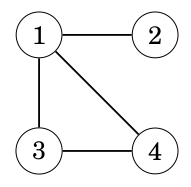
\includegraphics[width=0.15\linewidth]{img/graph_matrix_1}
		\label{fig:graphmatrix1}
	\end{figure}

	tiene tres árboles de expansión:
	
	\begin{figure}[h!]
		\centering
		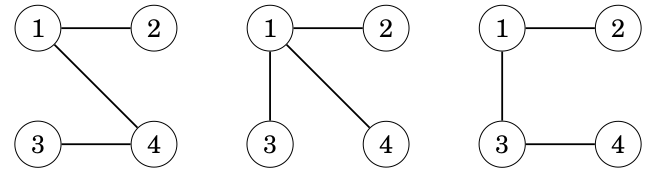
\includegraphics[width=0.5\linewidth]{img/graph_matrix_2}
		\label{fig:graphmatrix2}
	\end{figure}

	Para calcular el número de árboles de expansión, construimos una matriz de Laplacean $L$, donde $L[i,i]$ es el grado del nodo $i$ y $L[i,j]=-1$ si hay una arista entre los nodos $i$ y $j$, y de lo contrario, $L[i,j] = 0$. La matriz de Laplace para el grafo anterior es la siguiente:
	
	$$
	L = \begin{bmatrix}
		3 & -1 & -1 & -1  \\
		-1 & 1  & 0 & 0 \\
		-1 & 0  & 2 & -1 \\
		-1 & 0  & -1 & 2
	\end{bmatrix}
$$	
	Se puede demostrar que el número de árboles generadores es igual al determinante de una matriz que se obtiene cuando eliminamos cualquier fila y cualquier columna de $L$. Por ejemplo, si eliminamos la primera fila y columna, el resultado es:
	
		$$
	det( \begin{bmatrix}
		
		 1  & 0 & 0 \\
		 0  & 2 & -1 \\
		 0  & -1 & 2
	\end{bmatrix}) = 3
	$$
	El determinante es siempre el mismo, independientemente de qué fila y columna
	quitar de $L$ . Tenga en cuenta que la fórmula de Cayley es un caso especial del teorema de Kirchhoff, porque en se aplica a un grafo completo de $n$ nodos.
	
		$$
	det(\begin{bmatrix}
		n-1 & -1 & \ldots & -1  \\
		-1 & n-1  & \ldots & -1 \\
		\vdots & \vdots  & \ddots & \vdots \\
		-1 & -1  & \ldots & n-1
	\end{bmatrix}) = n^{n-2}
	$$	
	
	\item Una recurrencia lineal es una función $f(n)$ cuyos valores iniciales son $f(0),f(1), \dots ,f(k-1)$ y los valores mayores se calculan recursivamente usando la fórmula
	
	$$f(n)= c_1f(n-1)+ c_2f(n-2) + \dots + c_kf(n-k)$$
	
	donde $c_1 , c_2 , \dots , c_k$ son coeficientes constantes.
	
	La programación dinámica se puede utilizar para calcular cualquier valor de $f(n)$ en O($kn$) tiempo calculando todos los valores de $f(0),f(1),\dots ,f(n)$ uno tras otro. Sin embargo, si $k$ es pequeño, es posible calcular $f(n)$ mucho más eficientemente en tiempo O($k^3 \log n$) usando operaciones matriciales.
	
	Un ejemplo sencillo de recurrencia lineal es la siguiente función que define los números de Fibonacci:
	$$\begin{tabular}{rl}
		f (0) = & 0  \\
		f (1) = & 1 \\
		f (n) =	& f ( n - 1) + f ( n - 2)  \\
	\end{tabular}$$ 

En este caso, $k = 2$ y $c_1 = c_2 = 1$.

Para calcular eficientemente los números de Fibonacci, representamos la fórmula de Fibonacci como una matriz cuadrada $X$ de tamaño $2 \times 2$, para la cual se cumple lo siguiente:

$$X \cdot \begin{bmatrix}
	f(i)  \\
	f(i+1) 
\end{bmatrix} = \begin{bmatrix}
f(i+1)  \\
f(i+2) 
\end{bmatrix}$$

Por lo tanto, los valores $f(i)$ y $f(i+1)$ se dan como \emph{entrada} para $X$, y $X$ calcula los valores $f(i+1)$ y $f(i+2)$ a partir de ellos. Resulta que dicha matriz es:

$$X = \begin{bmatrix}
	0 & 1  \\
	1 & 1 
\end{bmatrix}$$

Por ejemplo:

$$ \begin{bmatrix}
	0 & 1  \\
	1 & 1 
\end{bmatrix} \cdot \begin{bmatrix}
f(5)  \\
f(6) 
\end{bmatrix} =\begin{bmatrix}
0 & 1  \\
1 & 1 
\end{bmatrix} \cdot  \begin{bmatrix}
5  \\
8 
\end{bmatrix} = \begin{bmatrix}
8  \\
13 
\end{bmatrix} $$

Por tanto, podemos calcular $f(n)$ usando la fórmula
$$ \begin{bmatrix}
	f(n)  \\
	f(n+1) 
\end{bmatrix} = X^n \cdot \begin{bmatrix}
f(0)  \\
f(1) 
\end{bmatrix} = \begin{bmatrix}
0 & 1  \\
1 & 1 
\end{bmatrix}^n \cdot  \begin{bmatrix}
0  \\
1 
\end{bmatrix} $$

Consideremos ahora el caso general donde f ( n ) es cualquier recurrencia lineal. Nuevamente, nuestro objetivo es construir una matriz X para la cual:
 $$ X \cdot \begin{bmatrix}
 	f ( i )  \\
 	f ( i+1 ) \\
 	\vdots \\
 	f(i+k-1) 
 \end{bmatrix} =   \begin{bmatrix}
 	f(i+1)  \\
 	f(i+2) \\
 	\vdots \\
 	f(i+k) 
 \end{bmatrix} $$
 Tal matriz es
 $$ X = 
 \begin{bmatrix}
 	0      &      1 &      0 &      0 & \ldots & 0  \\
 	0      &      0 &      1 &      0 & \ldots & 0  \\
 	0      &      0 &      0 &      1 & \ldots & 0  \\
 	\vdots & \vdots & \vdots & \vdots & \ddots & \vdots  \\
 	0      &      0 &      0 &      0 & \ldots & 1  \\
 	c_k    & c_{k-1}&c_{k-2} &c_{k-3} & \ldots & c_{1}
 \end{bmatrix}$$
 En las primeras $k-1$ filas, cada elemento es $0$ excepto que un elemento es $1$. Estas filas reemplazan $f(i)$ con $f(i+1)$, $f(i+1)$ con $f(i+2)$, y así en. La última fila contiene los coeficientes de recurrencia para calcular el nuevo valor $f(i+k)$.
 Ahora, $f(n)$ se puede calcular en tiempo O($k^3\log n$) usando la fórmula:
 $$  \begin{bmatrix}
 	f ( n )  \\
 	f ( n+1 ) \\
 	\vdots \\
 	f(n+k-1) 
 \end{bmatrix} = X^n \cdot  \begin{bmatrix}
 f(0)  \\
 f(1) \\
 \vdots \\
 f(k-1) 
\end{bmatrix} $$
\end{itemize}
\section{Complejidad}
Para ver la complejidad vamos a analizarla por cada una de las operaciones abordadas

\begin{enumerate}
	\item \textbf{Traspuesta:} Para esta operación  su complejidad temporal es O($n^2$) siendo $n$ las dimensiones de la matriz. Mientras en la espacial tenemos O($n^2$) en la matriz original y O($n^2$) en la matriz traspuesta.
	\item \textbf{Suma:} Para esta operación  su complejidad temporal es O($n^2$) siendo $n$ las dimensiones de la matriz. Mientras en la espacial tenemos O($2n^2$)  por las dos matrices que se suman y O($n^2$) en la matriz resultado.
	\item \textbf{Multipicación:}
	\begin{itemize}
		\item \textbf{Por un valor:} Para esta operación su complejidad temporal es O($n^2$) siendo $n$ las dimensiones de la matriz. Mientras en la espacial tenemos O($n^2$) en la matriz original y O($n^2$) en la matriz resultado.
		\item \textbf{Por una matriz:}  Para esta operación su complejidad temporal es O($n\times m \times l $) siendo $n$ filas de la matriz $A$, $m$ las columnas y filas de $A$ y $B$ respectivamente mientras $l$ las columnas de $B$. En caso de matrices cuadradas ambas burno es evidente que la complejidad es O($n^3$). En cuanto a la complejidad espacial es O($n\cdot m + m\cdot l+ n\cdot l$) por tomando en cuenta las tres matrices.
	\end{itemize}
	\item \textbf{Matriz identidad:} Para esta operación tanto su complejidad temporal como espacial es O($n^2$) siendo $n$ las dimensiones de la matriz.
	\item \textbf{Potencia:} Es operación tiene una complejidad de temporal de O($n^3\log k$) siendo $n$ las dimensiones de la matriz y $k$ el exponente que se desea elevar la matriz. En cuanto a la complejidad espacial tiene la matriz que se le desea calcular la potencia que sería O($n^2$) y otro O($n^2$) en la matriz que se almacena el resultado 
	\item \textbf{Determinante:} Es operación tiene una complejidad de temporal de O($n^3$) siendo $n$ las dimensiones de la matriz. En cuanto a la complejidad espacial tiene la matriz que se le desea calcular el determinante que sería O($n^2$)
	\item \textbf{Rango:} Es operación tiene una complejidad de temporal de O($n^3$) siendo $n$ las dimensiones de la matriz. En cuanto a la complejidad espacial tiene la matriz que se le desea calcular el rango que sería O($n^2$) y un vector cuya complejidad espacial es O($n$.)
\end{enumerate}
\section{Ejercicios}
A continuación una lista de los ejercicios que se pueden resolver aplicando los contenidos abordados en la presente guía:

\begin{itemize}
	\item \href{https://cses.fi/problemset/task/1722}{CSES - Fibonacci Numbers}
	\item \href{https://dmoj.uclv.edu.cu/problem/secnum}{DMOJ - Secuencia numerada de lápices}
	\item \href{https://dmoj.uclv.edu.cu/problem/fibonaccicalculatio}{DMOJ - Fibonacci Calculation}
	\item \href{https://cses.fi/problemset/task/1096/}{CSES - Throwing Dice}
	\item \href{https://cses.fi/problemset/task/1723/}{CSES - Graph Paths I}
	\item \href{https://cses.fi/problemset/task/1724/}{CSES - Graph Paths II}
	\item \href{https://www.codechef.com/problems/CSTREE}{CodeChef - Complement Spanning Trees}
	\item \href{https://acm.timus.ru/problem.aspx?space=1&num=1041}{Timus - 1041 - Nikifor}
\end{itemize}

\end{document}